\documentclass[11pt]{article}
\usepackage[letterpaper]{geometry}

%Used to split pages into two columns, IE the truth tables
\usepackage{multicol}

%Used to place figures
\usepackage{graphicx}
\usepackage{float}

%Used so that multi-line caption text is centered instead of left-aligned
\usepackage[center]{caption}

%Used to squish TOC
\usepackage{setspace}

%Used to show code nicely formatted
\usepackage{listings}
\usepackage{color}

%Used for Showing Mathematical Proofs
\usepackage{amsmath,amsthm,amssymb}

%Used for tables
\usepackage{array}
\usepackage{booktabs}

%Used for canceling terms in Math
\usepackage{cancel}

\definecolor{dkgreen}{rgb}{0,0.6,0}
\definecolor{gray}{rgb}{0.5,0.5,0.5}
\definecolor{mauve}{rgb}{0.58,0,0.82}

\lstset{frame=tb,
	language=Java,
	aboveskip=3mm,
	belowskip=3mm,
	showstringspaces=false,
	columns=flexible,
	basicstyle={\small\ttfamily},
	numbers=none,
	numberstyle=\tiny\color{gray},
	keywordstyle=\color{blue},
	commentstyle=\color{dkgreen},
	stringstyle=\color{mauve},
	breaklines=true,
	breakatwhitespace=true,
	tabsize=3
}

%Used to include the signatures sheet
\usepackage{pdfpages}

\title{EENG490\linebreak \linebreak Integrated Oscilloscope/Logic Analyzer/Signal Generator}
\author{Jeremy Munson, Braeden Bryant}
\geometry{top=.8in, bottom=.8in, left=.8in, right=.8in}

\setlength{\parindent}{0em}
\setlength{\parskip}{.5em}
\setlength{\floatsep}{-20px}
\setlength{\textfloatsep}{-20px}

\begin{document}
	
	%COVER SHEET%
	\thispagestyle{empty}
	\begin{center}
		\vspace*{1cm}
		\Huge
		\textbf{EENG490, Capstone:\linebreak \linebreak Integrated Oscilloscope/Logic Analyzer/Signal Generator}
		\vspace{0.5cm}
		\LARGE
		\vspace{1.5cm}

		Jeremy Munson\quad
		Braeden Reed\quad
		Bryant Clark\quad

		\vfill

		
\includegraphics[width=0.4\textwidth]{EWULogo.png}

		\Large

		Eastern Washington University

		Electrical and Computer Engineering Department

		Student Report

		Mar 21, 2024

	\end{center}
	\newpage
	\pagenumbering{arabic}
	%END COVER SHEET%

	\addcontentsline{toc}{section}{Table Of Contents}
	\setcounter{tocdepth}{2}
	\begin{spacing}{0.1}
		\tableofcontents
		\listoffigures
	\end{spacing}
	\newpage

	\section{Abstract}
	This document is a draft outlining the research and development done for the Integrated Oscilloscope/Logic Analyzer/Signal Generator project and fulfills the first half of the senior capstone project requirement for the EENG department of Easter Washington University. 


	\section{Proposal}
	\subsection{Introduction}
In engineering laboratories and industrial settings, electrical engineers make use of a wide variety of test equipment. The large number of devices becomes difficult to manage on a desktop, especially in a University setting where twenty or more stations need to fit into a single room. We will construct a product that is able to cover all of the common test-equipment and lab needs for electrical engineering education with a single device that is still capable enough to fit into industrial use.

	\subsection{Motivation}
Often, a proper electrical engineering workstation would need many devices: Bench power supplies, digital multimeters, signal generators, an LCR meter, logic analyzers, and oscilloscopes are the most common pieces of equipment...

	\subsection{Constraints}
	\begin{itemize}
		\item Time
			\begin{itemize}
			\item College classes will take time away from the final project.
			\item Downtime waiting on part delivery.
			\end{itemize}
		\item The project isn't intended to have a high cost but the intended customizability means there is a limit to how cheap the project will be.
		\item Part availability shouldn't be too much of a problem however certain aspects of the design require parts with the right specifications.
	\end{itemize}
	\subsection{Costs}
	It will cost Jeremy way more than he wants to admit.
	\subsection{Deliverables}
	It'll make you breakfast and run your feet.
	\subsection{Conclusion}
	The Better Than Elvis project will provide valuable experience to use going forward with our education. The multifaceted nature of the project will push us in areas of design and engineering that we have yet to be tested in while potentially being the first step in creating a new and better product for universities to use for education.
	/\section{Introduction}

	\section{Team Organization}
	\subsection{Background}
	\subsubsection{Jeremy Munson}
		PCB Design Experience
	\subsubsection{Bryant}
		Programming Internship
	\subsubsection{Braeden}
		
	\subsection{Responsibilities}
	\subsubsection{Jeremy Munson}
		\begin{itemize}
			\item PCB Design
			\item FPGA Programming
			\item Assembly
			\item Part Ordering
		\end{itemize}

	\subsubsection{Braeden}
		\begin{itemize}
			\item Power Supplies
			\item Breaboard pin function selection
			\item Embedded Programming
		\end{itemize}
		
	\subsubsection{Bryant}
		\begin{itemize}
			\item EZ USB
			\item User Space Software
			\item Embedded programming
		\end{itemize}

	\section{Initial Research}
	\subsection{Project Feasibility}
	Wanting a product to exist is all well and good, but if we don't consider the many moving parts needed to build a working product then we could be left with nothing but a dream, and no substance.
	
	\subsubsection{Oscilloscope}
	The oscilloscope really is the center-piece of the design. Preliminary research shows than often, oscilloscope manufacturers resort to ASIC\footnote{Application Specific Integrated Circuit} silicon for the Analog-to-digital conversion components. Since we don't have the millions of dollars and years of engineer time to design an ASIC, we will need to find a readily available chip that can perform the ADC conversions at an acceptable rate for an oscilloscope.
	
	Jeremy spent many hours scouring over part catalogs, looking for a suitable chip that is cost-effective. Fortunately, a line of chips ... HMCAD
	\subsection{Similar Products}
	There are several products on the market that attempt to address the same goal, but they each fall short in one or more ways.
	\subsubsection{NI Instruments Elvis III}
		\begin{itemize}
			\item Costs over \$3000
			\item Oscilloscope updates at 0.5hz
			\item 50-ohm signal generator, but incapable of driving 50-ohm terminated load
			\item Slow Interface
			\item 20 second DMM settling time
		\end{itemize}

	\section{Project Overview}
	\subsection{Design Criteria}
	yep.
	\subsection{Overview}
	\subsection{Architecture Block Diagram}
	Figure (\ref{fig:architecture.block_diagram}) Shows the high level overview of how the parts will connect. Figure (\ref{fig:architecture.tile_diagram}) Shows how the Analog output tile board will function.

	\begin{figure}[H]
		\centering
		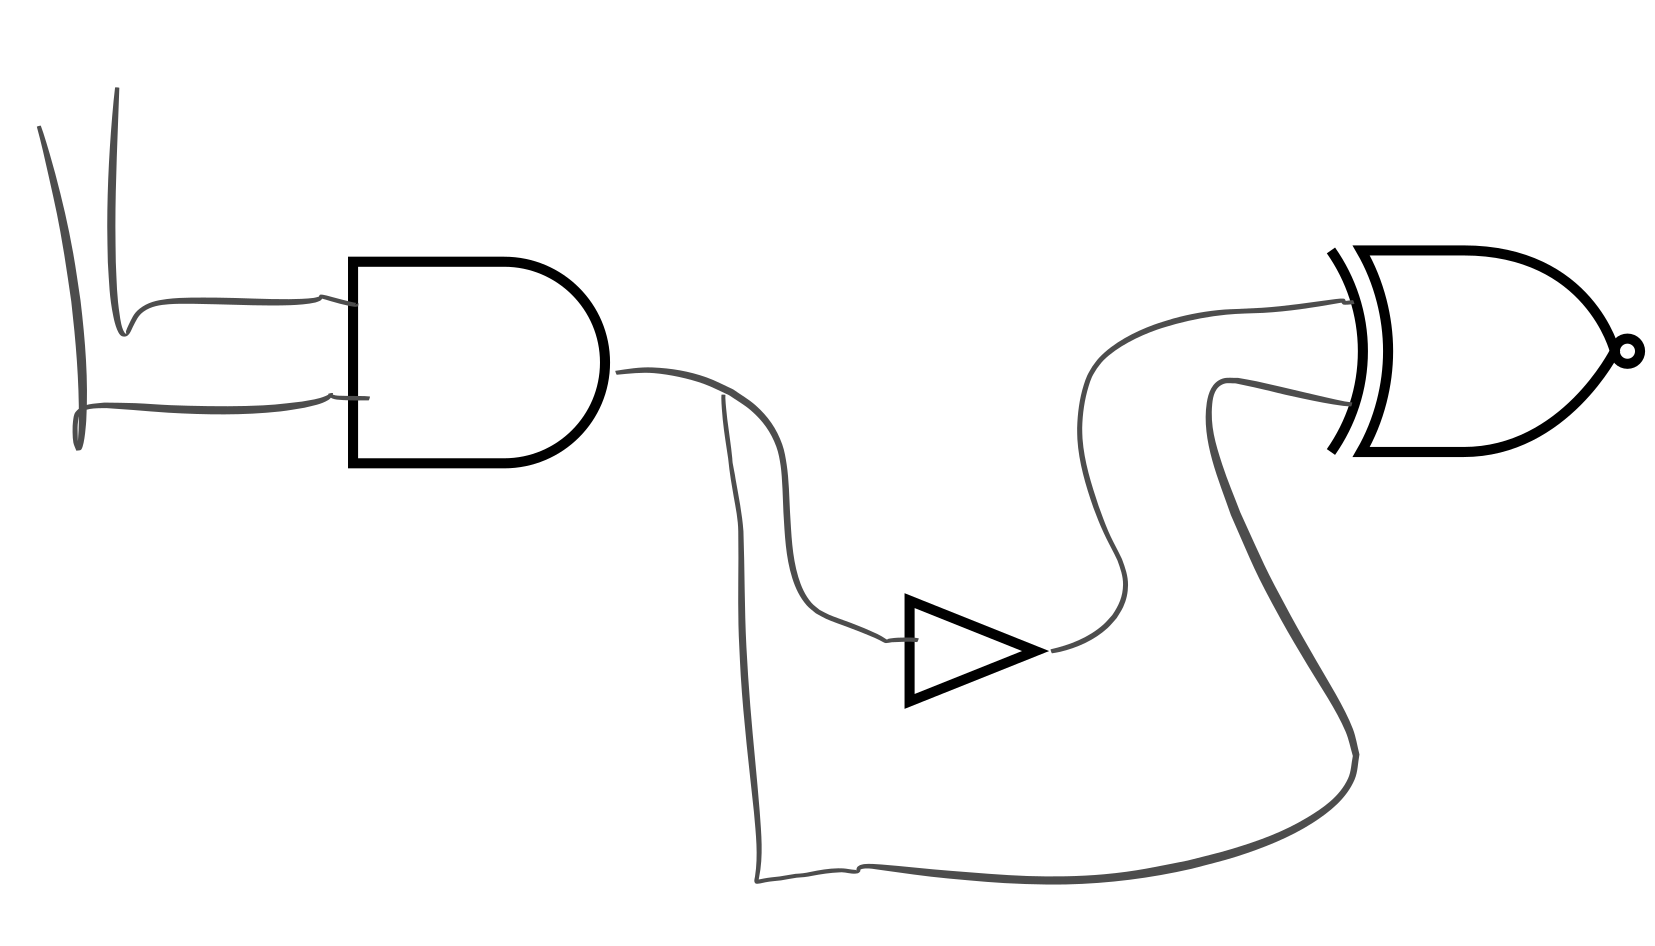
\includegraphics[width=0.8\linewidth]{images/architecture.block_diagram.png}
		\caption{Block diagram showing high-level design}
		\label{fig:architecture.block_diagram}
		\vspace{15px}
	\end{figure}

	\begin{figure}[H]
		\centering
		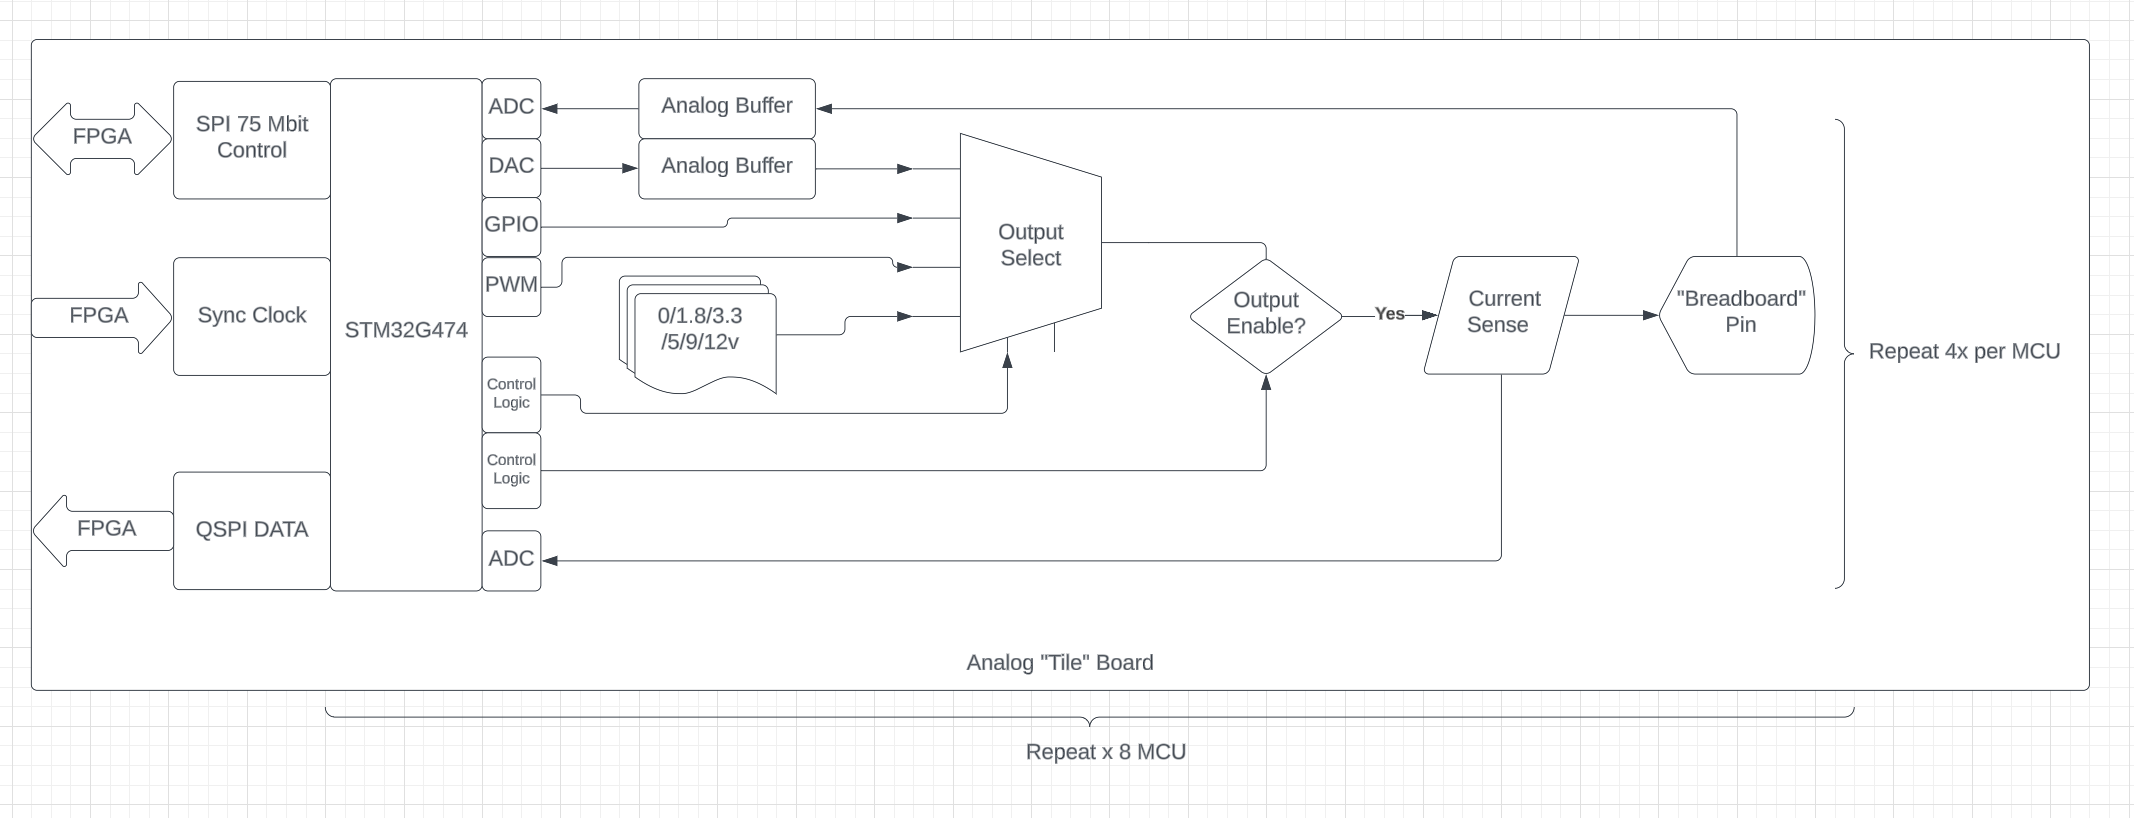
\includegraphics[width=0.8\linewidth]{images/architecture.tile_diagram.png}
		\caption{Analog "IO" Tile Block Diagram}
		\label{fig:architecture.tile_diagram}
		\vspace{15px}
	\end{figure}
	\subsection{Interfaces}
	\subsubsection{USB}
	The design was intended to communicate over USB 3.0, to provide a high-bandwidth connection to the computer. Because the EZ USB software became unavailable partway through the project, what we presented did not have the USB interface functional. Going forward, it is likely that Infineon will make the software available again, perhaps after some outside pressure. The actual software aspect of using the USB interface is very short: We are to use an existing driver and only have to write a few hundred lines of code to aggregate and forward packets from multiple sources.

	\subsubsection{QSPI, OSPI}
	The individual analog tile boards are to communicate with either the FPGA or EZ USB over OSPI (Octal SPI) or QSPI (Quad SPI). This allows sufficient bandwidth to the computer to capture the entirety of the sampled data; allowing capture of waveform lengths only limited by the connected computer's memory. Since the EZ USB could not be made functional in time for the demonstration, the QSPI functionality remained proven, but not used for the demo.
	
	The Frequency of this interface is up to 166mhz, with at least 50mhz necessary to achieve the full data rate of the device. Because digital signals are made of many harmonics much higher than the base frequency of the signal, we must make extra considerations in the design. This requires the use of impedance matched transmitters, receivers, and cable. The system was designed to use 90 ohm impedance on the PCB traces, and have swappable termination/matching resistors so that the device could be tuned. The cable to be used is 0.025 inch pitch ribbon cable with signals in a GSGSG... pattern - one ground between each signal, and the end signals as grounds. This creates a consistent electromagnetic environment for the signals. The cable did not come with an impedance spec for this condition, but applying the formulas for impedance of a microstrip as a rough approximation yielded an expected impedance of $\approx80\Omega$. The choice of 90 ohm traces, terminators, and matching resistors reflects that it is generally better to overshoot the impedance a little than undershoot.
	
	Another effect is the transmission delay in the cable and pcb traces. Although this effect isn't strongly prevalent in these signal speeds, all PCB traces for the OSPI and QSPI signals were length matched within 0.2mm using the PCB design software.
	
	\subsubsection{Backup: UART}
	Since the EZ USB part of the project became blocked, we still needed a way to communicate with the host computer to relay data. Fortunately, in the development board design we did include connections for a backup UART connection. This backup connection runs at a rate of 16Mbaud, which is very fast for UART without synchronization. Effort was made to maintain signal integrity by isolating this signal from other sources of interference. 
	
	Additionally, most operating systems do not have the capability to set a baud rate above 4Mbaud easily. For this purpose, Jeremy wrote a program "baud set" that interacts with the target operating systems and sets this baud rate in spite of operating system limitations.
	
	The Additional speed is very nescessary, as even a sample rate of 1Msps requires 10Mbaud to fully transmit it's data.
	
	\subsection{Schedule}
	Intended start and end times for the tasks necessary to the project. Ideally three weeks left at the end for debugging, polishing, and finalizing the project.
	\subsubsection{Gantt Chart}
			\begin{figure}[H]
				\centering
				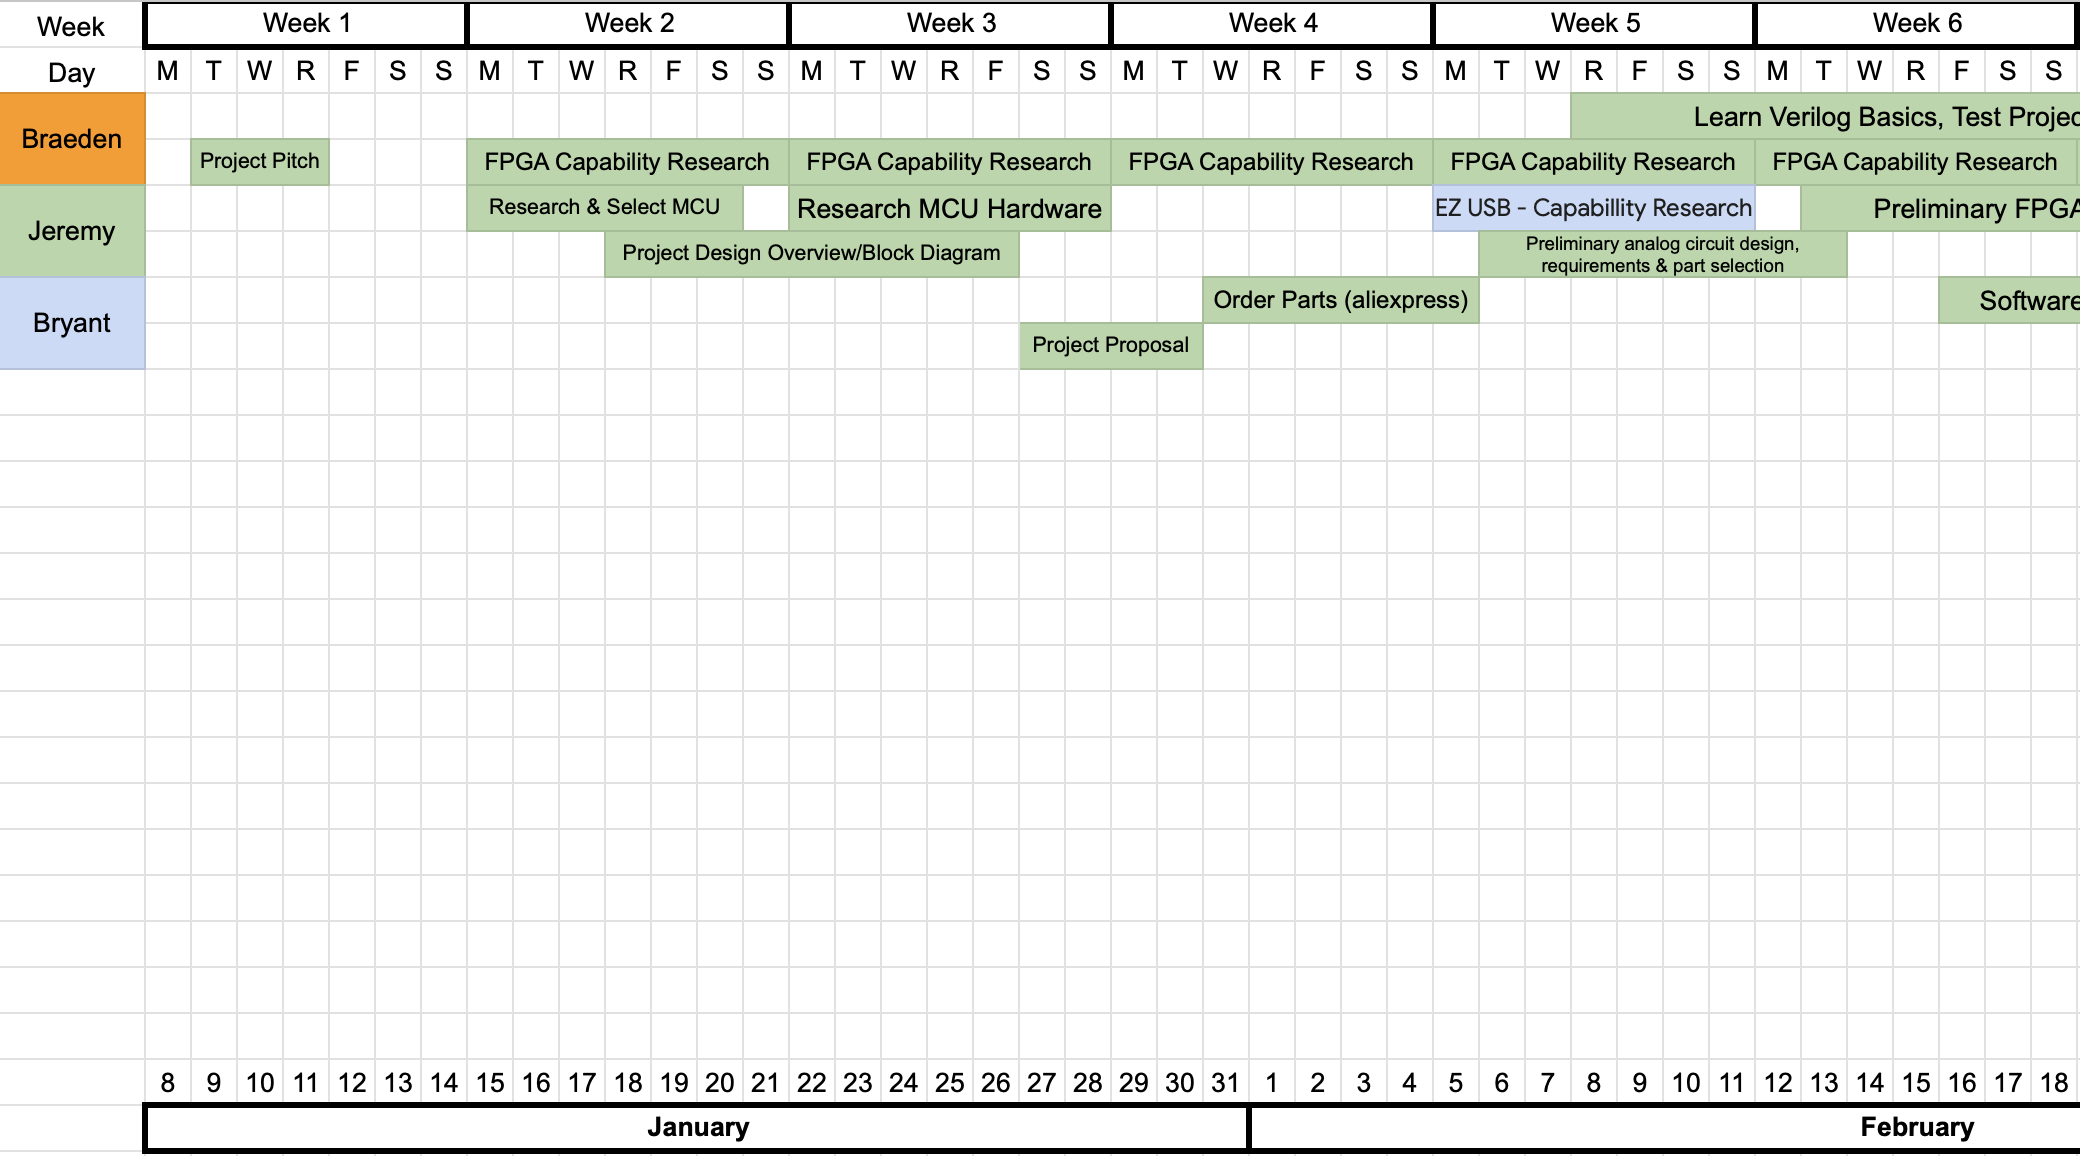
\includegraphics[width=0.8\linewidth]{images/GANTT1.png}
				\caption{GANTT Winter Weeks 1-6}
				\label{fig:ngscope-client}
				\vspace{15px}
			\end{figure}
			\begin{figure}[H]
				\centering
				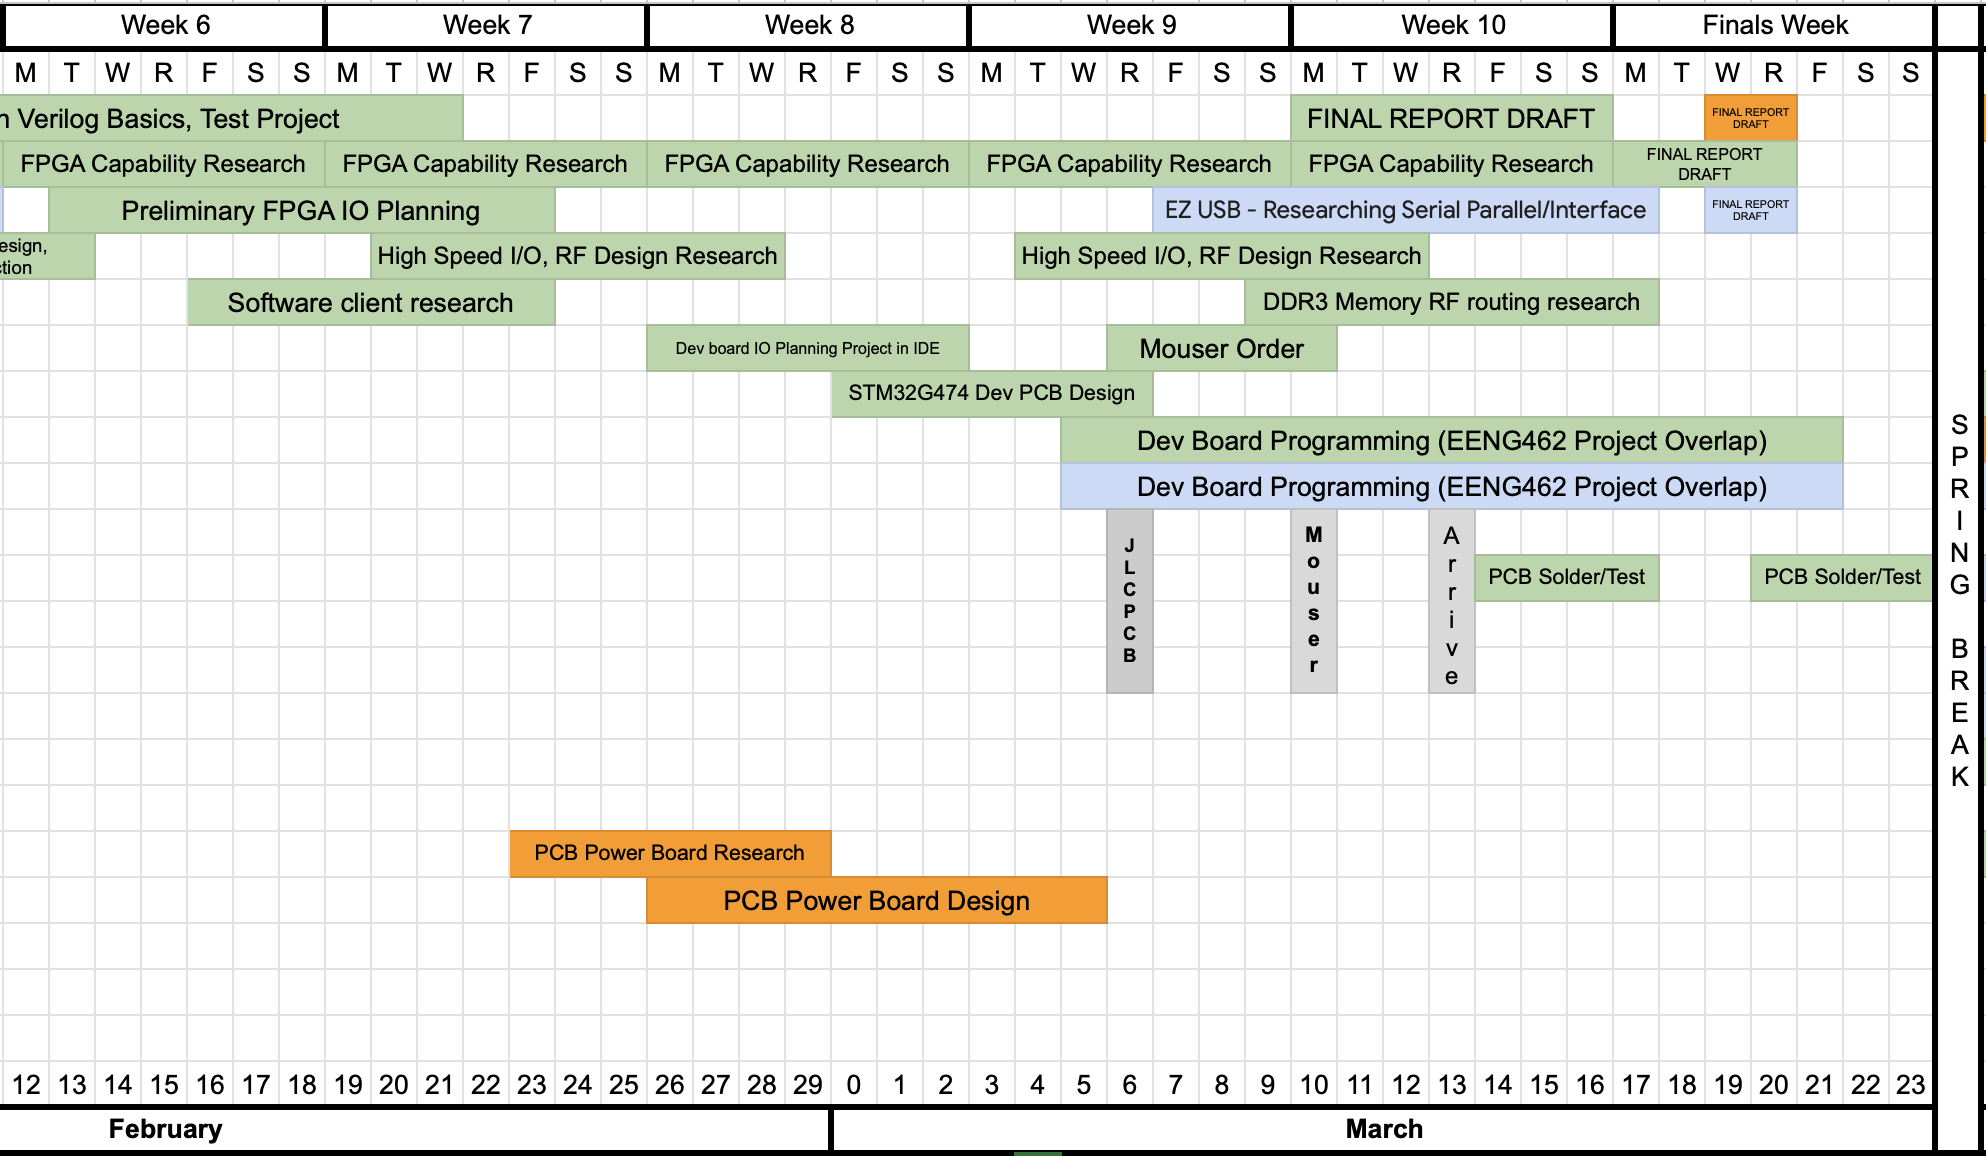
\includegraphics[width=0.8\linewidth]{images/GANTT2.png}
				\caption{GANTT Winter Weeks 6-11}
				\label{fig:ngscope-client}
				\vspace{15px}
			\end{figure}
			\begin{figure}[H]
				\centering
				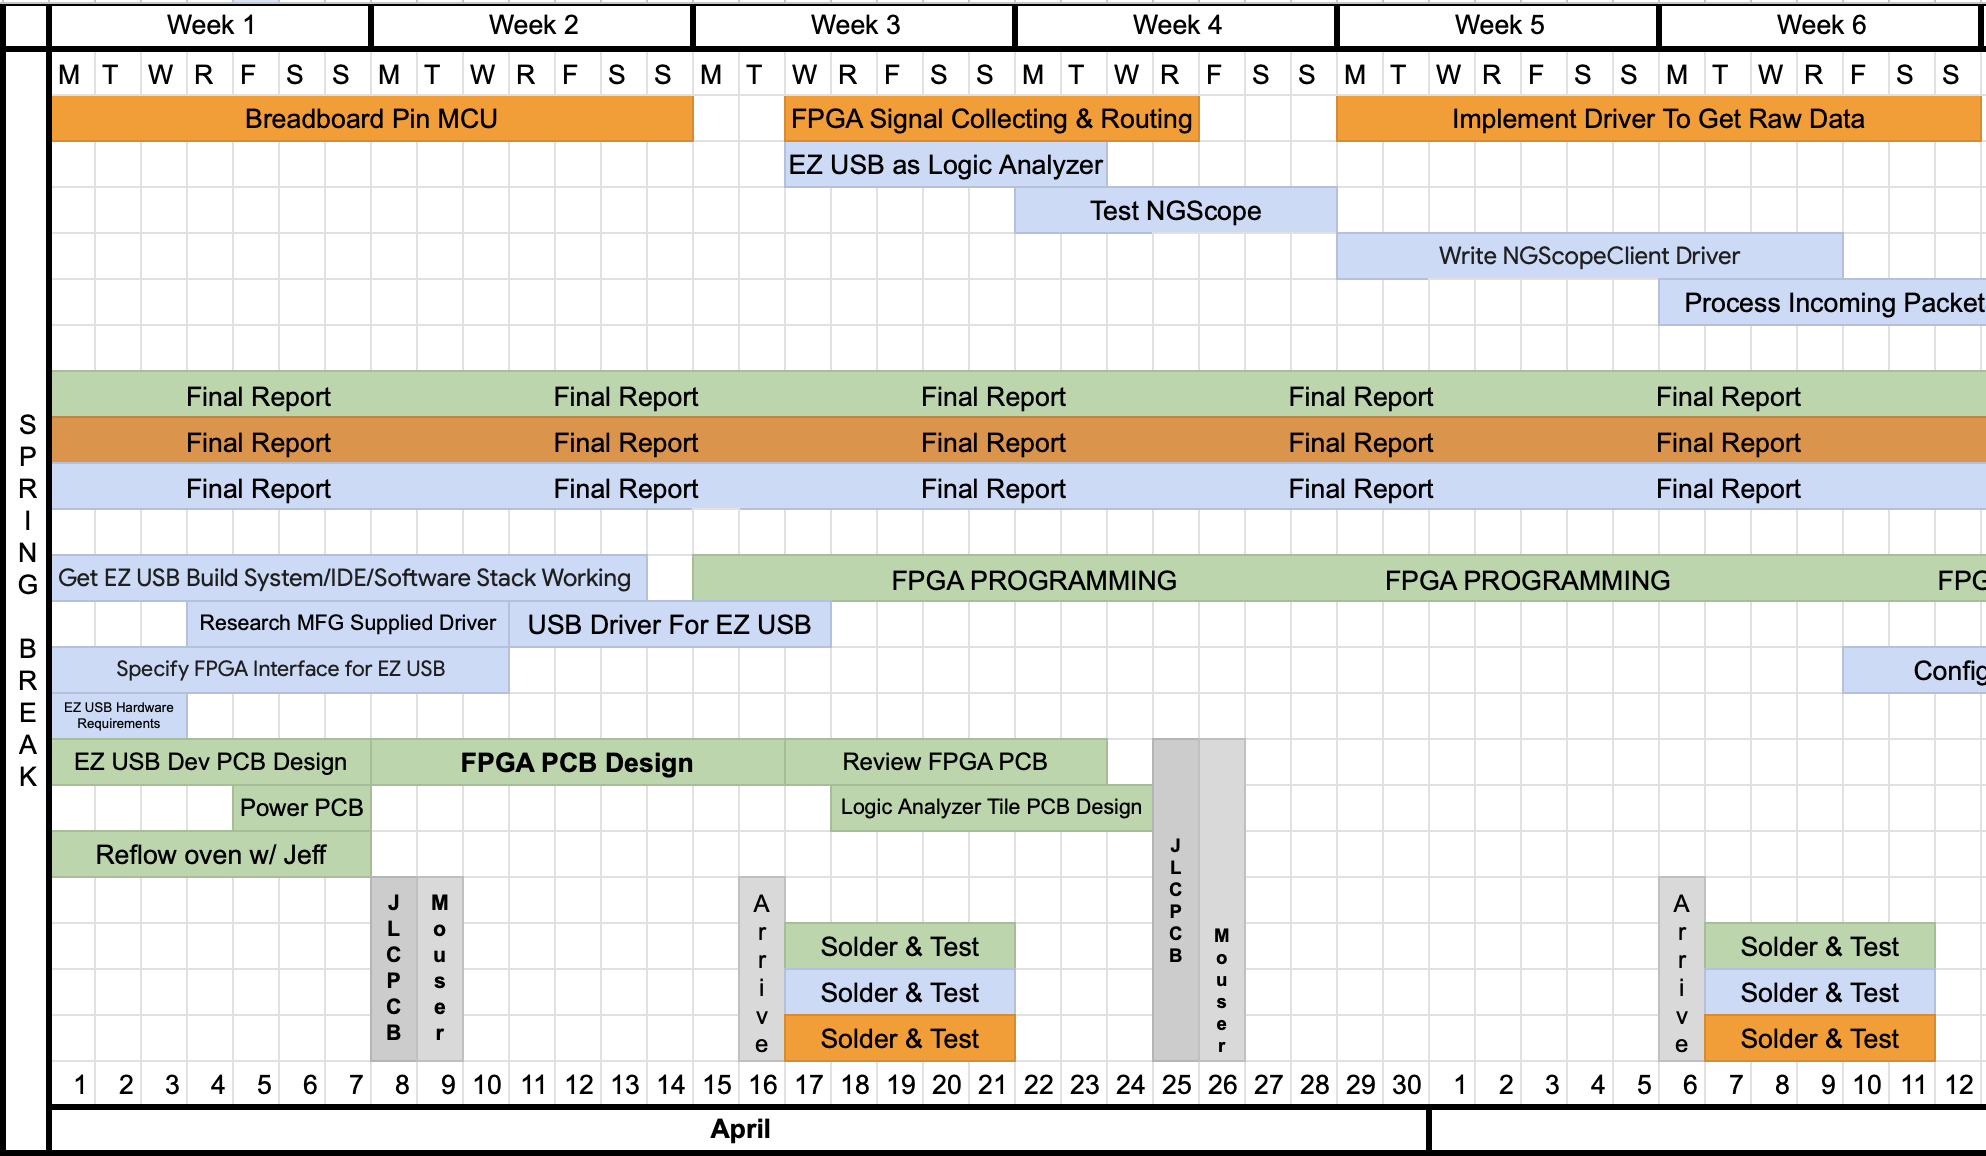
\includegraphics[width=0.8\linewidth]{images/GANTT3.png}
				\caption{GANTT Spring Weeks 1-6}
				\label{fig:ngscope-client}
				\vspace{15px}
			\end{figure}
			\begin{figure}[H]
				\centering
				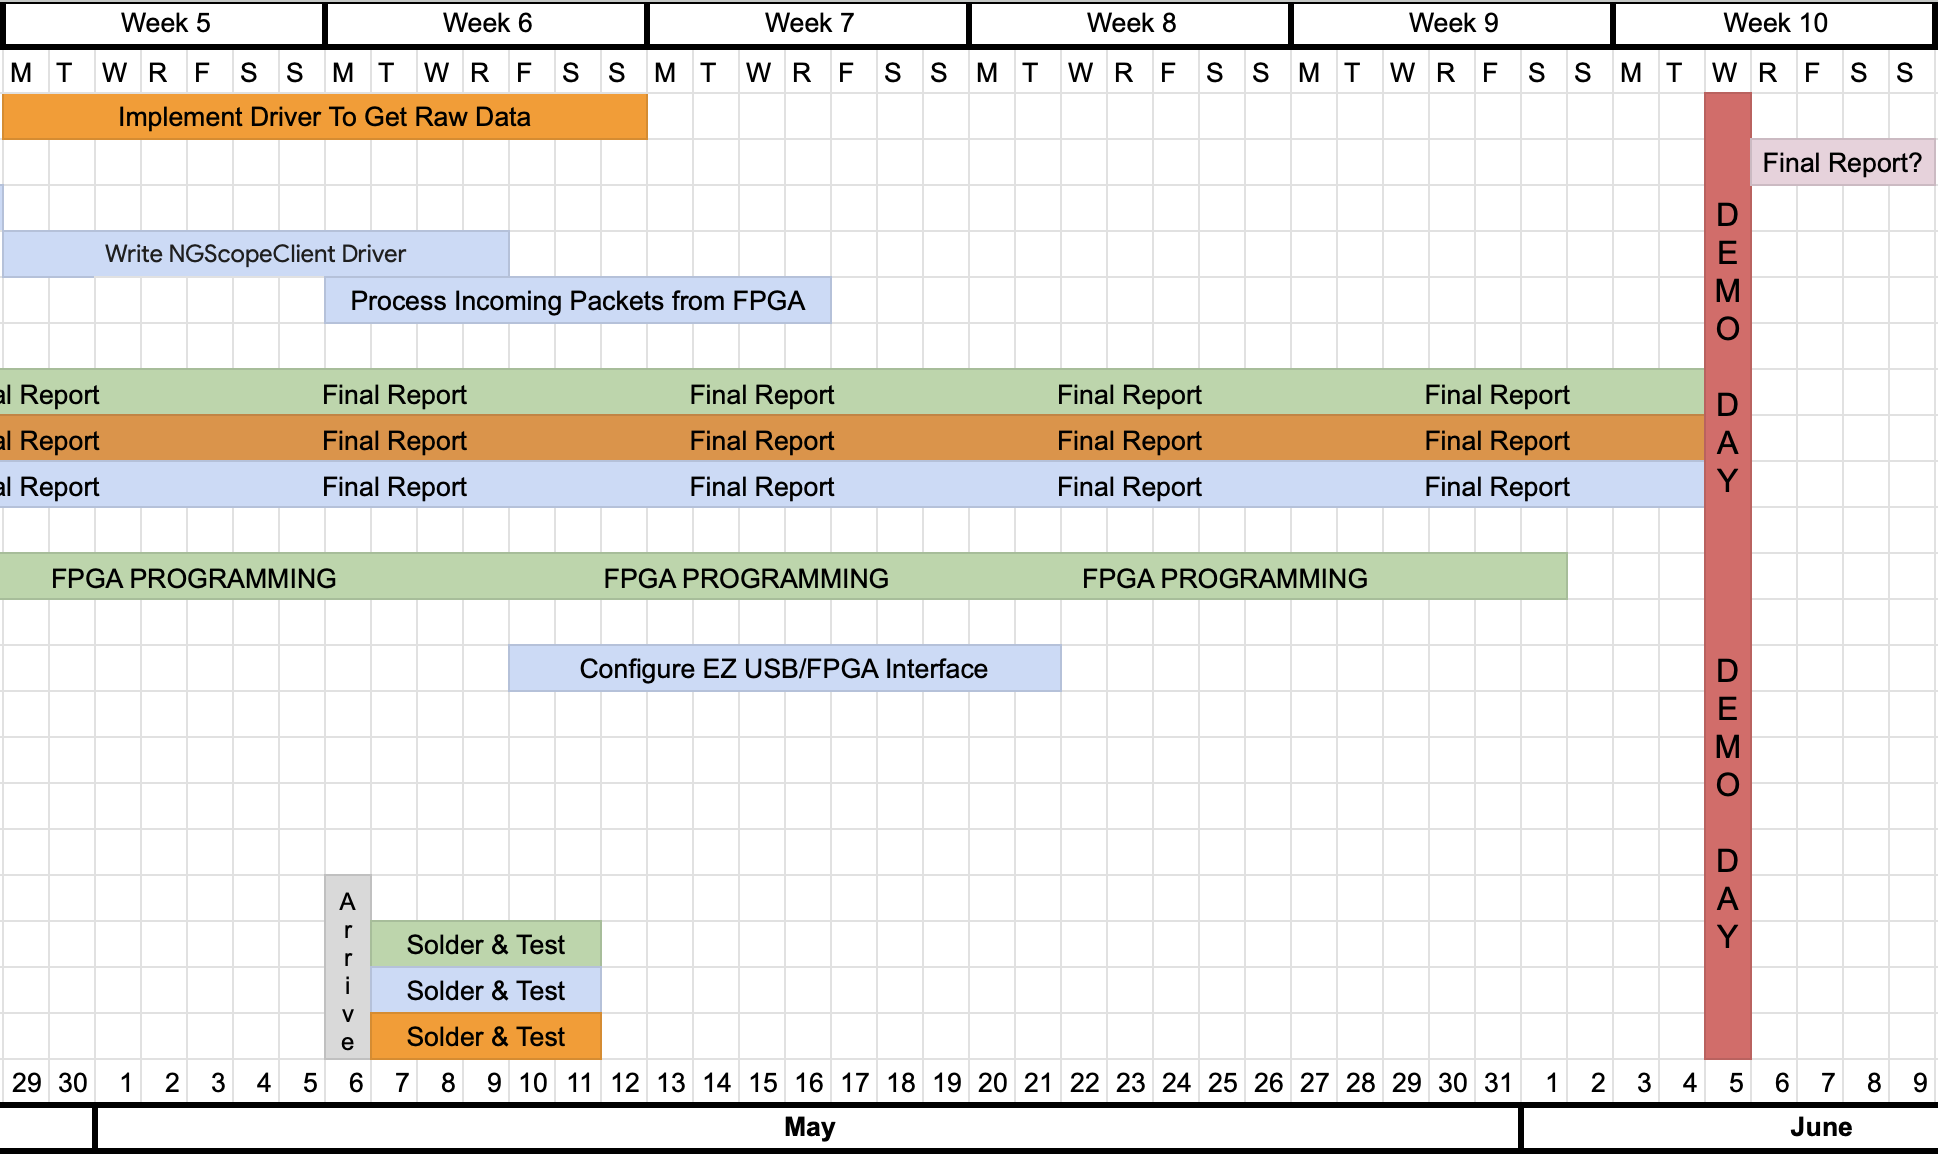
\includegraphics[width=0.8\linewidth]{images/GANTT4.png}
				\caption{GANTT Spring Weeks 5-10}
				\label{fig:ngscope-client}
				\vspace{15px}
			\end{figure}
			

	\section{Research of Proposed Solutions}
	\subsection{Gsps ADC: HMCAD2011}
	The core of the oscilloscope design, the Analog To Digital converter takes the analog voltages that we want to measure. This part will be capable of high speed data collection, with standard sampling rates. This will provide a relatively cheap yet effective means for data collection.
	\subsection{Signal Generator}
	An unlikely source of capable signal generator chips: Display drivers! There are numberous triple-channel DAC chips that are intended to drive displays at a low(ish) cost. We can re-purpose one of these display driver chips as a three-channel signal generator, instead of a 3-color pixel control.
	\subsection{USB 3.2 Gen 1 Interface}
	The all-important interface that allows data to be delivered to a computer to be analyzed: the USB 3 interface. Our project is extremely data intensive so we had to find a solution that would have high bandwidth at a low cost. We decided to use Infineon's EZ-USB™ FX3. It is relitively affordable and it can transfer data at five gigabits per second. It can be configured for most common peripheral communication proticals such as I²C, I²S, UART, and SPI but we will be configuring it to run, effectively, our own communication protical because that allows us to use the full 32-bit wide parrallel bus. This will allow us to get the high data rates that we need to get all the data from the FPGA to the computer application.
	\subsection{Artix-7 FPGA}
	The glue that brings everything together. No other (feasible) device would be capable of aggregating the veritable firehose of data that we will be collecting. The FPGA forms the center of our design.
	\subsection{STM32, Providing ADC and DAC for logic analyzer}
The STM32G474RE is a critical part of the design. It has several ADC's and DAC's at its disposal with a variety of useful configurations. Four 12-bit unbuffered internal DAC channels with 15 MSPS allows the board incredibly fast output, providing accurate data display for high speed processes. Five 12-bit ADC's provide the board with means to sample and gather data.
	\subsection{Power Supply}
There are multiple aspects to the power supply: Power from the wall, then powr to the devices.
	\subsection{Bread Board Unit}
	While test equipment often has BNC connectors, or test leads, or banana plug jacks to connect wires to your project, we would like to take a different approach. We want to have a breadboard that can be switched onto all of the possible connections at each pin in software. This lets up place components down on a breadboard, use jumper wires to form the connections, then apply a stimulus with the signal generator or power rail functionality using software. This allows exploring a wide variety of stimuli quickly. Since every pin will also be an analog logic analyzer channel we will be able to visualize the operation of the entire circuit at once.
	\subsection{NGScopeClient}
	Once the data is gathered from the hardware it needs to be presented in a readable manner. to do this we originally planned to build our own front end application. Bryant has experience in that and we did not know of any open source front ends that we liked. However, during Jeremy's hardware research he spoke extensively with an engineer in the feild who happened to mention ngscopeclient.org to him. When we saw it, we were sold. It is an open source platform that works acrossed OSX, Windows, and Linux. It can be interacted with using a C/C++ backend and it has beutiful graphics as shown in figure 2. These features fit our application perfectly.
	
		\begin{figure}[H]
		\centering
		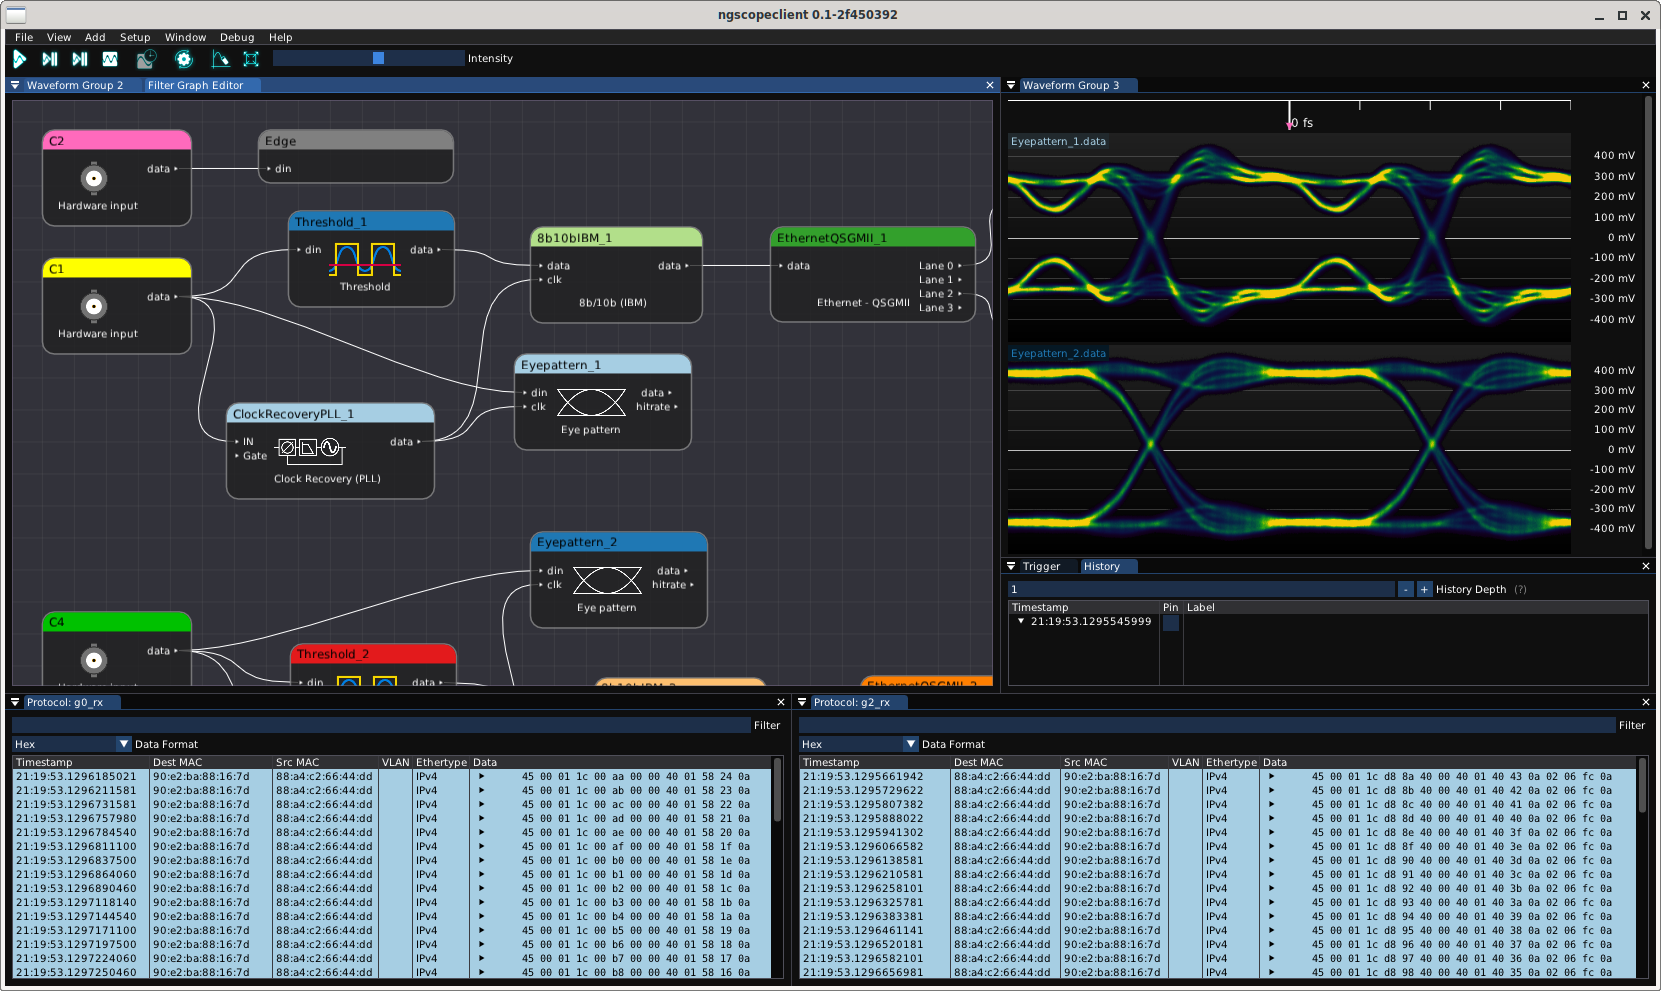
\includegraphics[width=0.8\linewidth]{images/ngscopeclient-intro.png}
		\caption{NGScopeClientGraphics [1]}
		\label{fig:ngscope-client}
		\vspace{15px}
	\end{figure}
	

	‌
	
	\section{References}
	
[1]“Streamline hardware test,” ngscopeclient. https://www.ngscopeclient.org 
‌

\end{document}
